\documentclass[letter,10pt]{article}
\usepackage[utf8]{inputenc}
\usepackage[english]{babel}
\usepackage{float}
\usepackage{graphicx}
\usepackage{caption}
\usepackage{subcaption}
\usepackage{amsmath}
\usepackage{multirow}
\usepackage{color}
\usepackage{tabularx}
\begin{document}

\section{Datasets}

\begin{figure}[H]
    \centering
    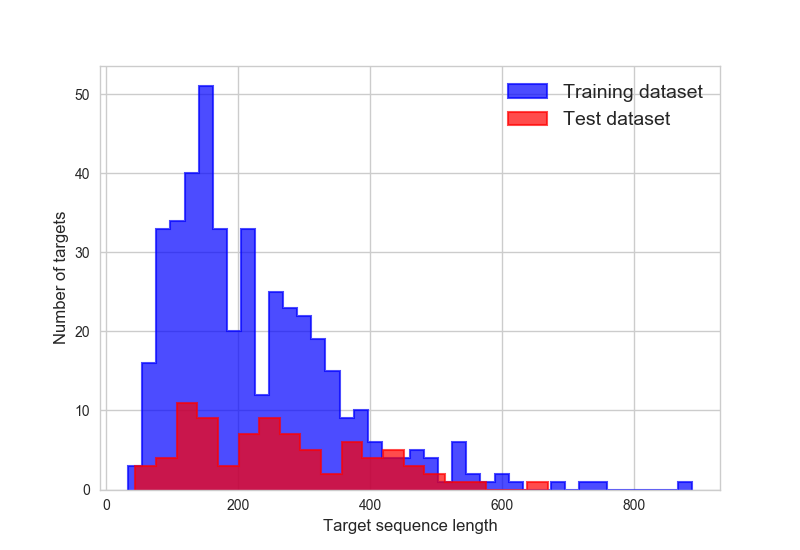
\includegraphics[width=\linewidth]{Fig/datasetLengthDistributions.png}
    \caption{Distributions of sequence lengths for targets in training set (blue) and test set (red).}
    \label{Fig:dataLengthDist}
\end{figure}

\begin{table}[H]
\begin{center}
\begin{tabular}{ c | c | l }
    
    Test set ID & Closest training set ID & E-value \\
    \hline
    T0768 & T0690 & $2.70\times 10^{-13}$ \\
    T0770 & T0645 & $1.79\times 10^{-13}$ \\
    T0772 & T0518 & $1.89\times 10^{-7}$ \\
    T0776 & T0707 & $3.98\times 10^{-5}$ \\
    T0783 & T0699 & $1.19\times 10^{-22}$ \\
    T0798 & T0308 & $9.57\times 10^{-6}$ \\
    T0813 & T0398 & $2.45\times 10^{-5}$ \\
    T0819 & T0636 & $8.66\times 10^{-15}$ \\
    T0854 & T0324 & $2.13\times 10^{-13}$ \\
\end{tabular}
%   
    \caption{Closest homolog sequences from the training set. A
    sequence pair is reported if at least one training sequence aligns
    to a test sequence with a blastp E-value less than $10^{-4}$. Only
    the top alignment is reported for each test sequence.}
%
\label{Tbl:datasetsSimilarity}
\end{center}
\end{table}


\begin{table}[H]
\begin{center}
\begin{tabular}{ l | l | l }

    Common family & Test set target & Train set targets \\
    \hline
    PF00795 & T0794 & T0542 \\ \hline
    PF13472 & T0776 & T0448, T0297, T0286, T0750 \\ \hline
    PF03807 & T0813 & T0398, T0393, T0702 \\ \hline
    PF00266 & T0801 & T0339, T0697 \\ \hline
    PF01128 & T0783 & T0699, T0420 \\ \hline
    PF07949 & T0780 & T0572 \\ \hline
    PF13577 & T0815 & T0752, T0736 \\ \hline
    PF12804 & T0783 & T0593, T0699, T0420 \\ \hline
    PF13242 & T0854 & T0371, T0341, T0303, T0324, T0330, T0329, T0418 \\ \hline
    PF13306 & T0768 & T0690, T0671, T0713, T0653 \\ \hline
    PF12741 & T0770 & T0664, T0645, T0532 \\ \hline
    PF00025 & T0798 & T0308 \\ \hline
    PF12872 & T0792 & T0549 \\ \hline
    PF03446 & T0813, T0851 & T0398, T0393, T0702 \\ \hline
    PF00155 & T0801, T0819 & T0591, T0636, T0436, T0697 \\ \hline
    PF13419 & T0854 & T0371, T0341, T0303, T0379, T0324, T0330, T0329, T0418, T0635 \\ \hline
    PF12680 & T0815 & T0451, T0475 \\ \hline
    PF06439 & T0772 & T0518 \\ \hline
    PF12771 & T0770 & T0664, T0645, T0532 \\ \hline
    PF08477 & T0798 & T0308 \\ \hline
    PF00657 & T0776 & T0297, T0286, T0679 \\ \hline
    PF00071 & T0798 & T0308 \\ \hline
    PF00702 & T0854 & T0303, T0324, T0330, T0329, T0418, T0635 \\ \hline
    PF01926 & T0798 & T0308 \\ \hline
    PF12697 & T0764 & T0672 \\ \hline
\end{tabular}
   
\caption{Targets from test and training sets that belong to the same Pfam
family \cite{finn2016pfam}, based on a HMMER search \cite{finn2015hmmer} with an
E-value cutoff of 1.0. With that cutoff, 403 of the 564 training
targets and 65 of the 83 test targets could be assigned
families. There are 25 families containing at least one test sequence
and one training sequence, involving a total of 16 test targets and 42
training targets. Each of the 25 families belongs to a distinct Pfam
clan.}
%
\label{Tbl:SharedPfam}
\end{center}
\end{table}

\begin{table}[H]
\begin{center}
\begin{tabular}{ l | l | l }

    Target & Has PDB & Has ECOD classification \\
    \hline
    T0773 &True &False\\
    T0820 &False &False\\
    T0823 &False &False\\
    T0824 &False &False\\
    T0827 &False &False\\
    T0835 &False &False\\
    T0836 &False &False\\
    T0838 &False &False\\
\end{tabular}
   
\caption{Targets from CASP11 that do not have corresponding PDB entries or ECOD classification.}
%
\label{Tbl:CASP11PDB_ECOD}
\end{center}
\end{table}


Figure \ref{Fig:foldsGraph} shows the classification of the test set
into ECOD groups. Branches drawn in black correspond to groups
containing structures from the training set as well. Branches drawn in
grey correspond to groups unique to the test set. Targets T0773,
T0797, and T0816 are excluded from the analysis because they have no
ECOD classification, and targets T0820, T0823, T0824, T0827, T0835,
and T0836 are excluded because they have no structure in the RCSB PDB.

Four architecture groups present overlap at all levels between the
training and test sets: ``a/b barrels'', ``beta duplicates or obligate
multimers'', ``a+b complex topology'', and ``a+b four layers''.

\begin{figure}[H]
    \centering
    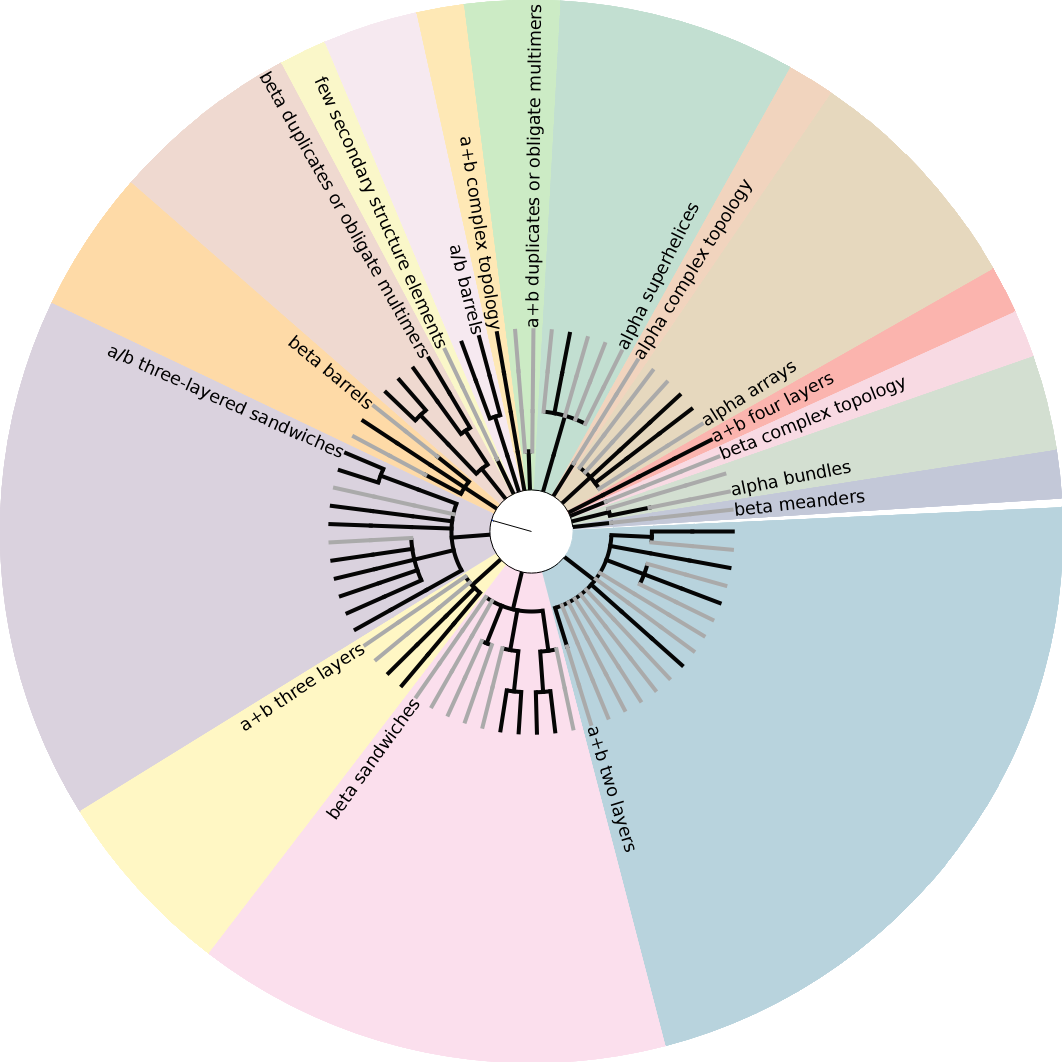
\includegraphics[width=\linewidth]{Fig/folds_graph.png}
%
    \caption{Classification of the test set structures into the lower
    four ECOD structural levels (from the center out): architecture
    (A), possible homology (X), homology (H), and topology (T). The
    names of the architecture types are shown in the outer circle of
    the diagram.
    The grey lines denote test set classes that have no
    respective representative in the training set. The black lines
    show the classes that have representatives in both training and
    test sets. We do not show the F-groups because they have litle
    overlap among the training and test sets.
}
%
    \label{Fig:foldsGraph}
\end{figure}

\section{Model}

\begin{table}[H]
\begin{center}
\makebox[0pt][c]{
\hskip-\footskip
\begin{tabularx}{0.8\paperwidth}{ l | l | c | c | c }

    Number & Layer name & Input dimentions & Output dimensions & Parameters \\
    \hline
    1&3D Convolution & $11\times 120\times 120\times 120$ & $16\times 118\times 118\times 118$ & 
                    Filter size: $3\times 3\times 3$ Stride: $1\times 1\times 1$\\
    2&ReLU & & & \\
    3&Max pooling & $16\times 118\times 118\times 118$ & $16\times 58\times 58\times 58$ & 
                    Filter size: $3\times 3\times 3$ Stride: $2\times 2\times 2$ \\
    \hline 
    4&3D Convolution & $16\times 58\times 58\times 58$ & $32\times 56\times 56\times 56$ & 
                    Filter size: $3\times 3\times 3$ Stride: $1\times 1\times 1$\\
    5&Batch normalization & & & \\
    6&ReLU & & & \\
    7&Max pooling & $32\times 56\times 56\times 56$ & $32\times 27\times 27\times 27$ & 
                    Filter size: $3\times 3\times 3$ Stride: $2\times 2\times 2$ \\
    \hline
    8&3D Convolution & $32\times 27\times 27\times 27$ & $32\times 25\times 25\times 25$ & 
                    Filter size: $3\times 3\times 3$ Stride: $1\times 1\times 1$\\
    9&Batch normalization & & & \\
    \textbf{10}&\textbf{ReLU} & & & \\
    11&3D Convolution & $32\times 25\times 25\times 25$ & $64\times 23\times 23\times 23$ & 
                    Filter size: $3\times 3\times 3$ Stride: $1\times 1\times 1$\\
    12&Batch normalization & & & \\
    13&ReLU & & & \\
    14&Max pooling & $64\times 23\times 23\times 23$ & $64\times 11\times 11\times 11$ & 
                    Filter size: $3\times 3\times 3$ Stride: $2\times 2\times 2$ \\
    \hline
    15&3D Convolution & $64\times 11\times 11\times 11$ & $128\times 9\times 9\times 9$ & 
                    Filter size: $3\times 3\times 3$ Stride: $1\times 1\times 1$\\
    16&Batch normalization & & & \\
    17&ReLU & & & \\
    18&3D Convolution & $128\times 9\times 9\times 9$ & $128\times 7\times 7\times 7$ & 
                    Filter size: $3\times 3\times 3$ Stride: $1\times 1\times 1$\\
    19&Batch normalization & & & \\
    20&ReLU & & & \\
    21&3D Convolution & $128\times 7\times 7\times 7$ & $256\times 5\times 5\times 5$ & 
                    Filter size: $3\times 3\times 3$ Stride: $1\times 1\times 1$\\
    22&Batch normalization & & & \\
    23&ReLU & & & \\
    24&3D Convolution & $256\times 5\times 5\times 5$ & $512\times 3\times 3\times 3$ & 
                    Filter size: $3\times 3\times 3$ Stride: $1\times 1\times 1$\\
    25&Batch normalization & & & \\
    26&ReLU & & & \\
    27&Max pooling & $512\times 3\times 3\times 3$ & $512\times 1\times 1\times 1$ & 
                    Filter size: $3\times 3\times 3$ Stride: $2\times 2\times 2$ \\
    \hline
    28&Reshape & $512\times 1\times 1\times 1$ & $512$ & \\
    \hline
    29&Linear & 512 & 256 & \\
    30&ReLU & & & \\
    31&Linear & 256 & 128 & \\
    32&ReLU & & & \\
    33&Linear & 128 & 1 & \\
    \hline

\end{tabularx}
\hskip\headheight
}
\caption{More details of the model architecture. The layer 10 is emphasised with the bold font, because its output was used in the Grad-CAM algorithm
in Analysis section of the paper.}
\label{Tbl:SuppModel}
\end{center}
\end{table}

\section{Training}
The rotations were sampled in the following way:
\begin{enumerate}
\item Select three random uniform values $u_1, u_2, u_3 \in [0,1]$
\item Construct quaternion from them
\begin{eqnarray}
q_0 = \sqrt(1-u_1) \sin(2\pi  u_2) \\
q_1 = \sqrt(1-u_1) \cos(2\pi  u_2) \\
q_2 = \sqrt(u_1) \sin(2\pi  u_3) \\
q_3 = \sqrt(u_1) \cos(2\pi  u_3) 
\end{eqnarray}
\item Construct corresponding rotation matrix
\end{enumerate}


The translations were sampled accoriding to the following algorithm:
\begin{enumerate}
\item Compute the bounding box of the atoms in the decoy
\item Shift protein such that the center of the bounding box corresponds to the frame origin 
\item Rotate protein using random uniform rotation
\item Calculate the maximum shift along each axis:
$$
D_k = \frac{1}{2}\max\left[ 0, \frac{S_k}{2.0} - \frac{B_k}{2.0} \right], k \in {x, y, z}
$$
where $S_k$ are input size along the axes x,y,z and $B_k$ are the bounding box sizes along the same axes.
\item Sample random uniform translation along each axis from the interval $[-\frac{D_k}{2}, \frac{D_k}{2}], k \in {x,y,z}$
\end{enumerate}


\begin{table}[H]
\begin{center}
\begin{tabular}{ l | l }

    Parameter & Value \\
    \hline
    Learning rate& 0.0003\\
    Learning rate decay& 0.01\\
    GDT\_TS threshold& 0.01\\
    Algorithm& Adam
    
\end{tabular}
\caption{Non-default training parameters}
%
\label{Tbl:TrainingParam}
\end{center}
\end{table}

\begin{figure}[H]
    \centering
    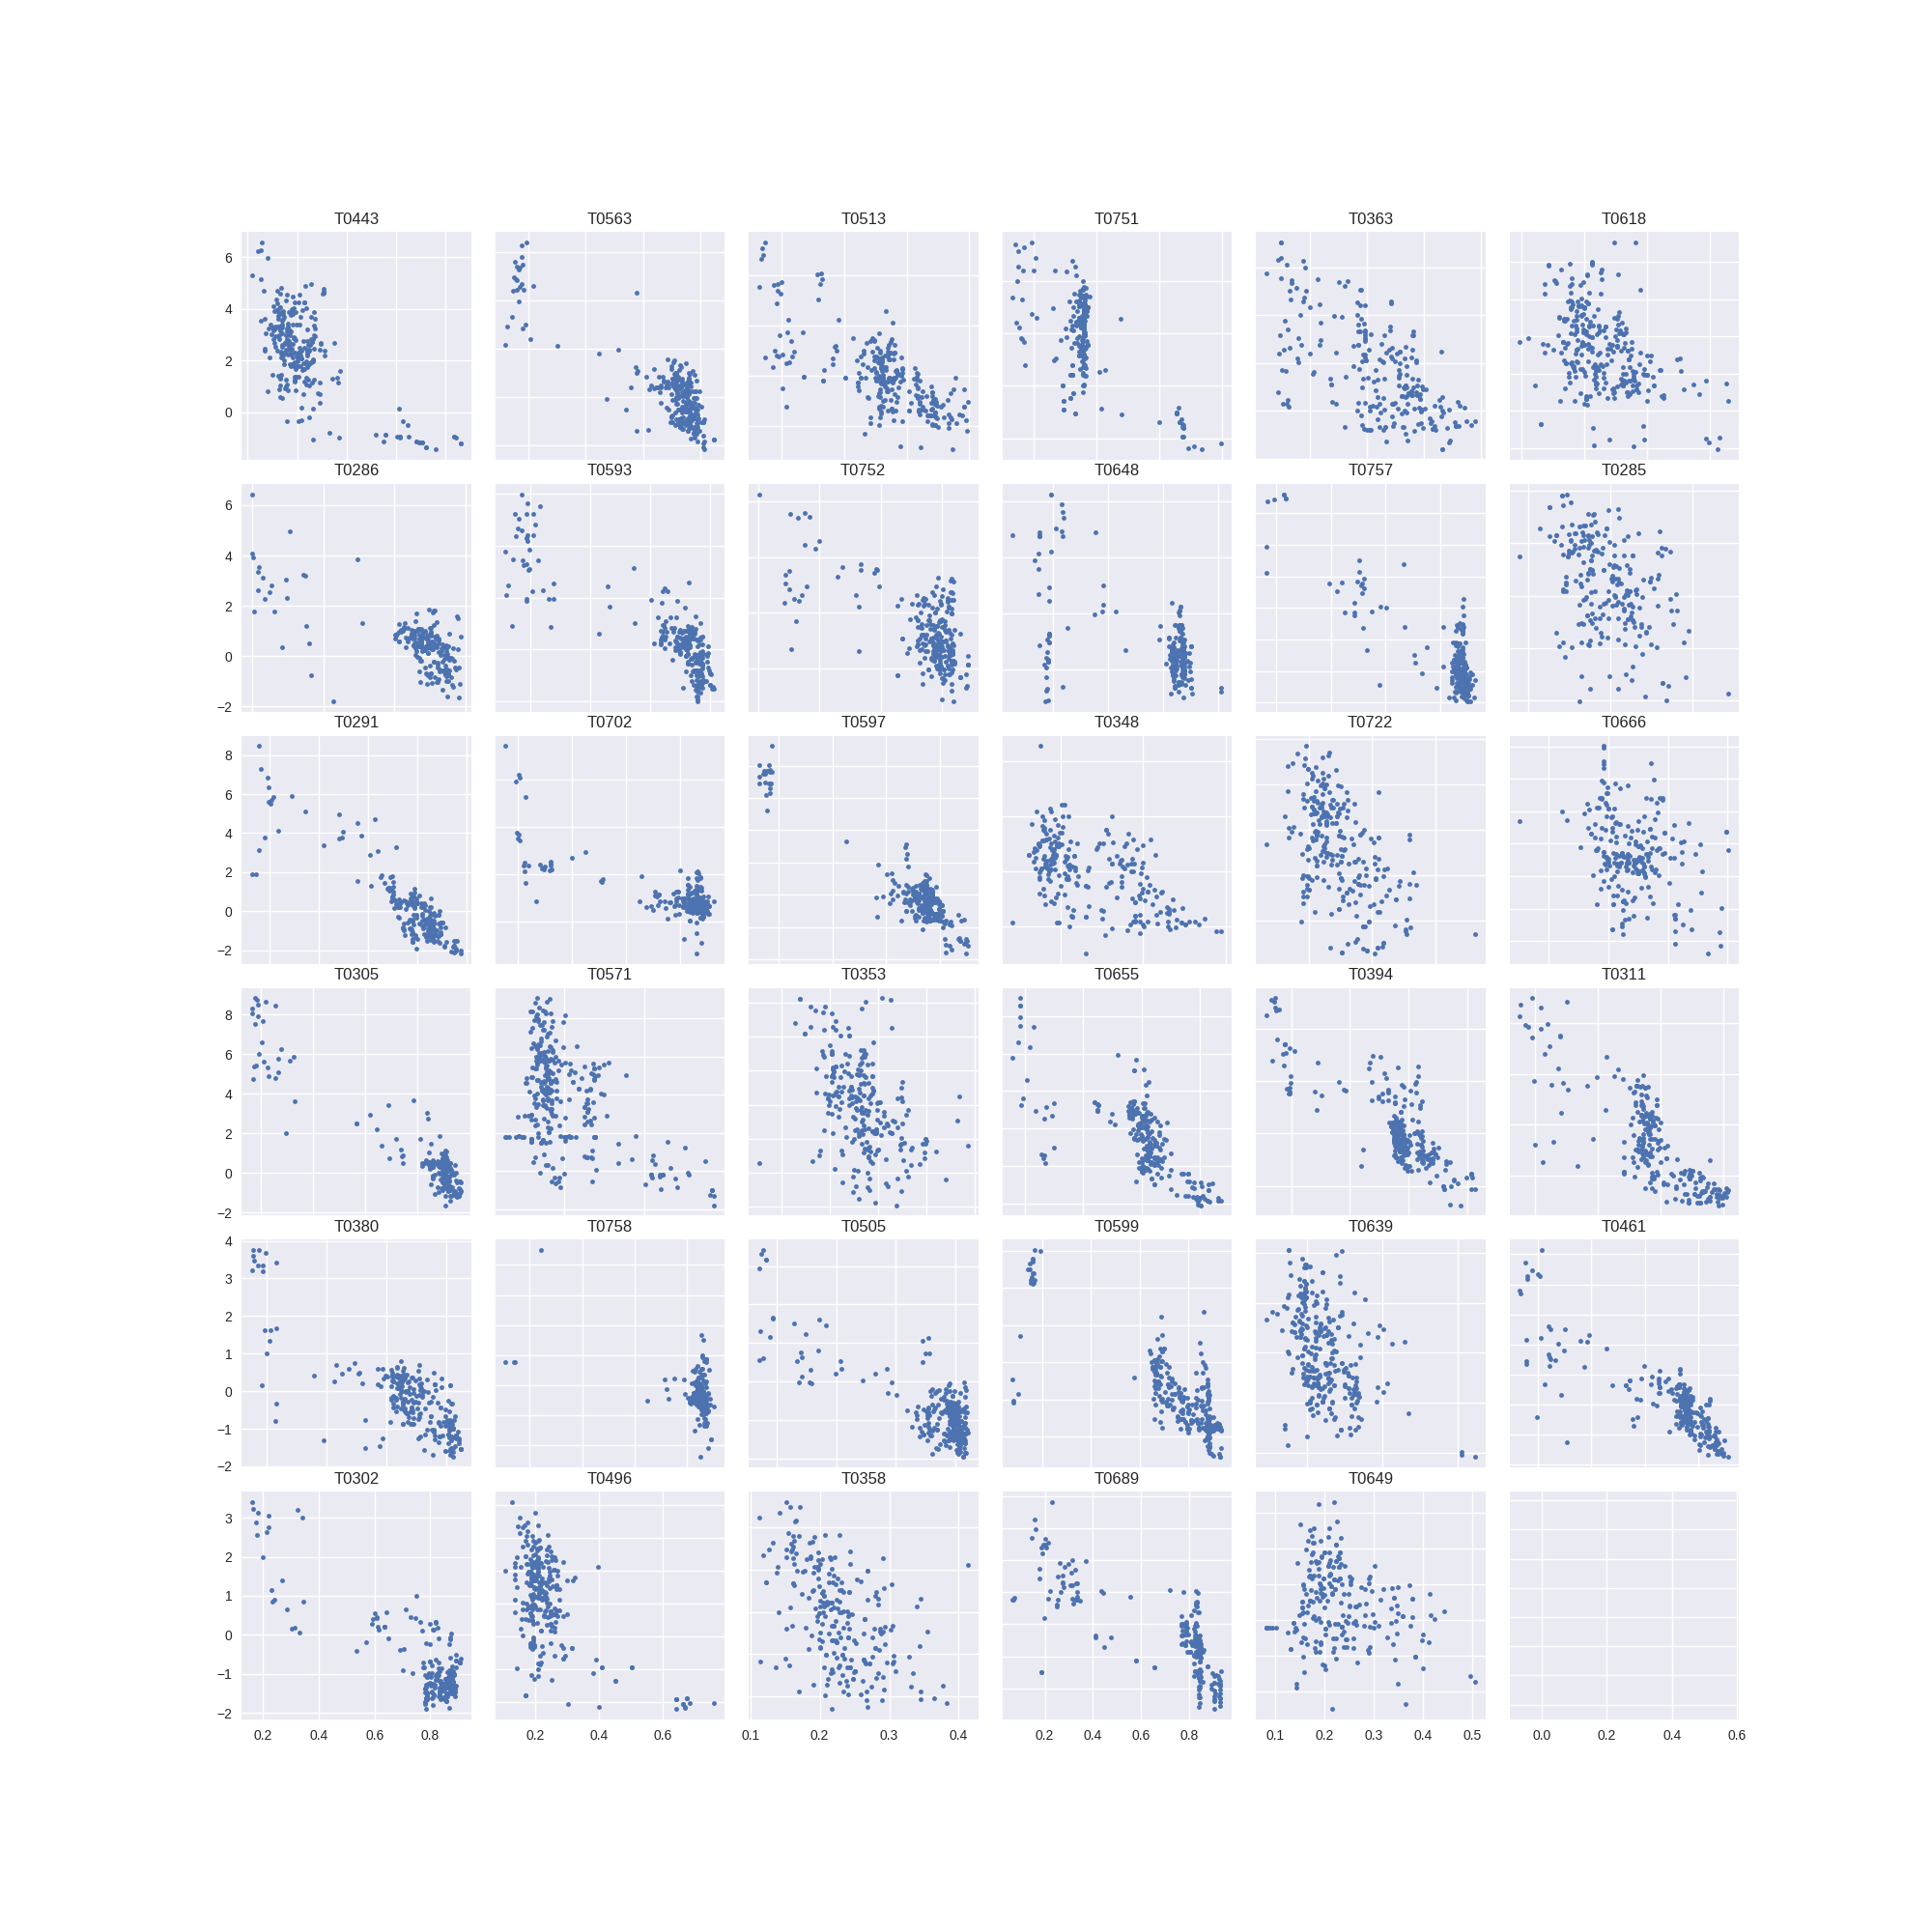
\includegraphics[width=\linewidth]{Fig/epoch40_funnels.png}
    \caption{Scoring funnels on the validation set at epoch 40. The score was sampled once using random rotation and translation.}
    \label{Fig:ValidationEpoch40}
\end{figure}

\section{Results}

\begin{figure}[H]
    \centering
    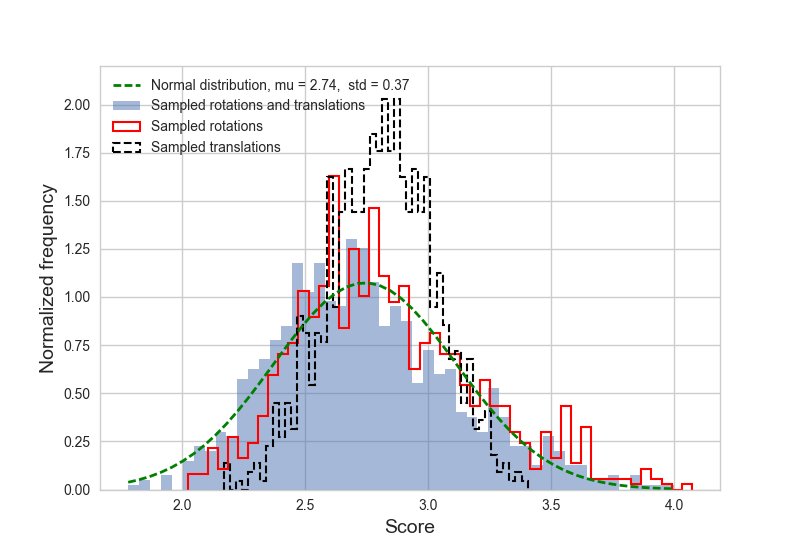
\includegraphics[width=\linewidth]{Fig/sampling_dist.eps}
%
    \caption{Distribution of the score of decoy FALCON\_EnvFold\_TS1
    for target T0832 under random translations and rotations. The
    distribution fits a normal distribution with an average $\mu =
    2.74$ and a standard deviation $\sigma = 0.37$ (shown in green
    dashed lines). The figure also shows the distributions of the
    score under rotations only (red lines) and under translations only
    (black dashed lines).}
%
    \label{Fig:ScoreDistribution}
\end{figure}

Figure~\ref{Fig:LossVsECOD} shows how the performance of each
algorithm is affected by the ECOD similarity of the structures used
for testing to those used for training. The test set in broken down
into 5 subsets:
\begin{itemize}
\item
``No overlap'', the structures for which there is no structure in the training set with 
the same ECOD ``A'' class (T0797 and T0773); see Fig.~\ref{Fig:summaryTable});
\item
``A'', the structures in the same A-group of at least one training
structure but not in the same X-group (T0759, T0763, T0769, etc.);
\item
``A+X'', the structures in the same X-group of at least one training
structure but not in the same H-group (T0760, T0761, T0765, etc.);
\item
``A+X+H+T'', the structures in the same T-group of at least one
training structure but not in the same F-group (T0762, T0766, T0767,
etc.);
\item
``A+X+H+T+F'', the structures in the same F-group of at least one
training structure (T0764, T0768, T0770, etc.).
\end{itemize}
%%% GL: Is this correct?
%
%%% GL: By the way, is Figure 1 correct for structures T0773, T0797,
%%% and T0816?  The ECOD information is available but the structures
%%% belong to A-groups not found in the training set?
%G: to do on server
%
% We expect the performance of any knowledge-based MQA method to
% increase as the structures used for testing become more similar to the
% structures used for training. By contrast, we would expect a purely
% first-principles method to show no increase in performance.
%
% Both our 3DCNN algorithm and the VoroMQA algorithm show marked
% performance gains as proteins become more similar to the training set,
% going from an average loss of around $0.10$ for ``no information''
% structures to an average loss of around $0.04$ for ``A+X+H+T+F''
% structures (see Fig.~\ref{Fig:LossVsECOD}).
%
% By comparison, algorithms ProQ2D and ProQ3D show modest performance
% gains (if any) and algorithm RWPlus shows a performance independent
% from structural similarity.
%
% Overall, these results suggest that the 3DCNN and VoroMQA methods make
% better use of structural information---and rely more on
% memorization---than the ProQ2D, ProQ3D, and RWPlus methods.
%%% GL: Does it make sense?
%G: to do on server


\begin{figure}[H]
    \centering
    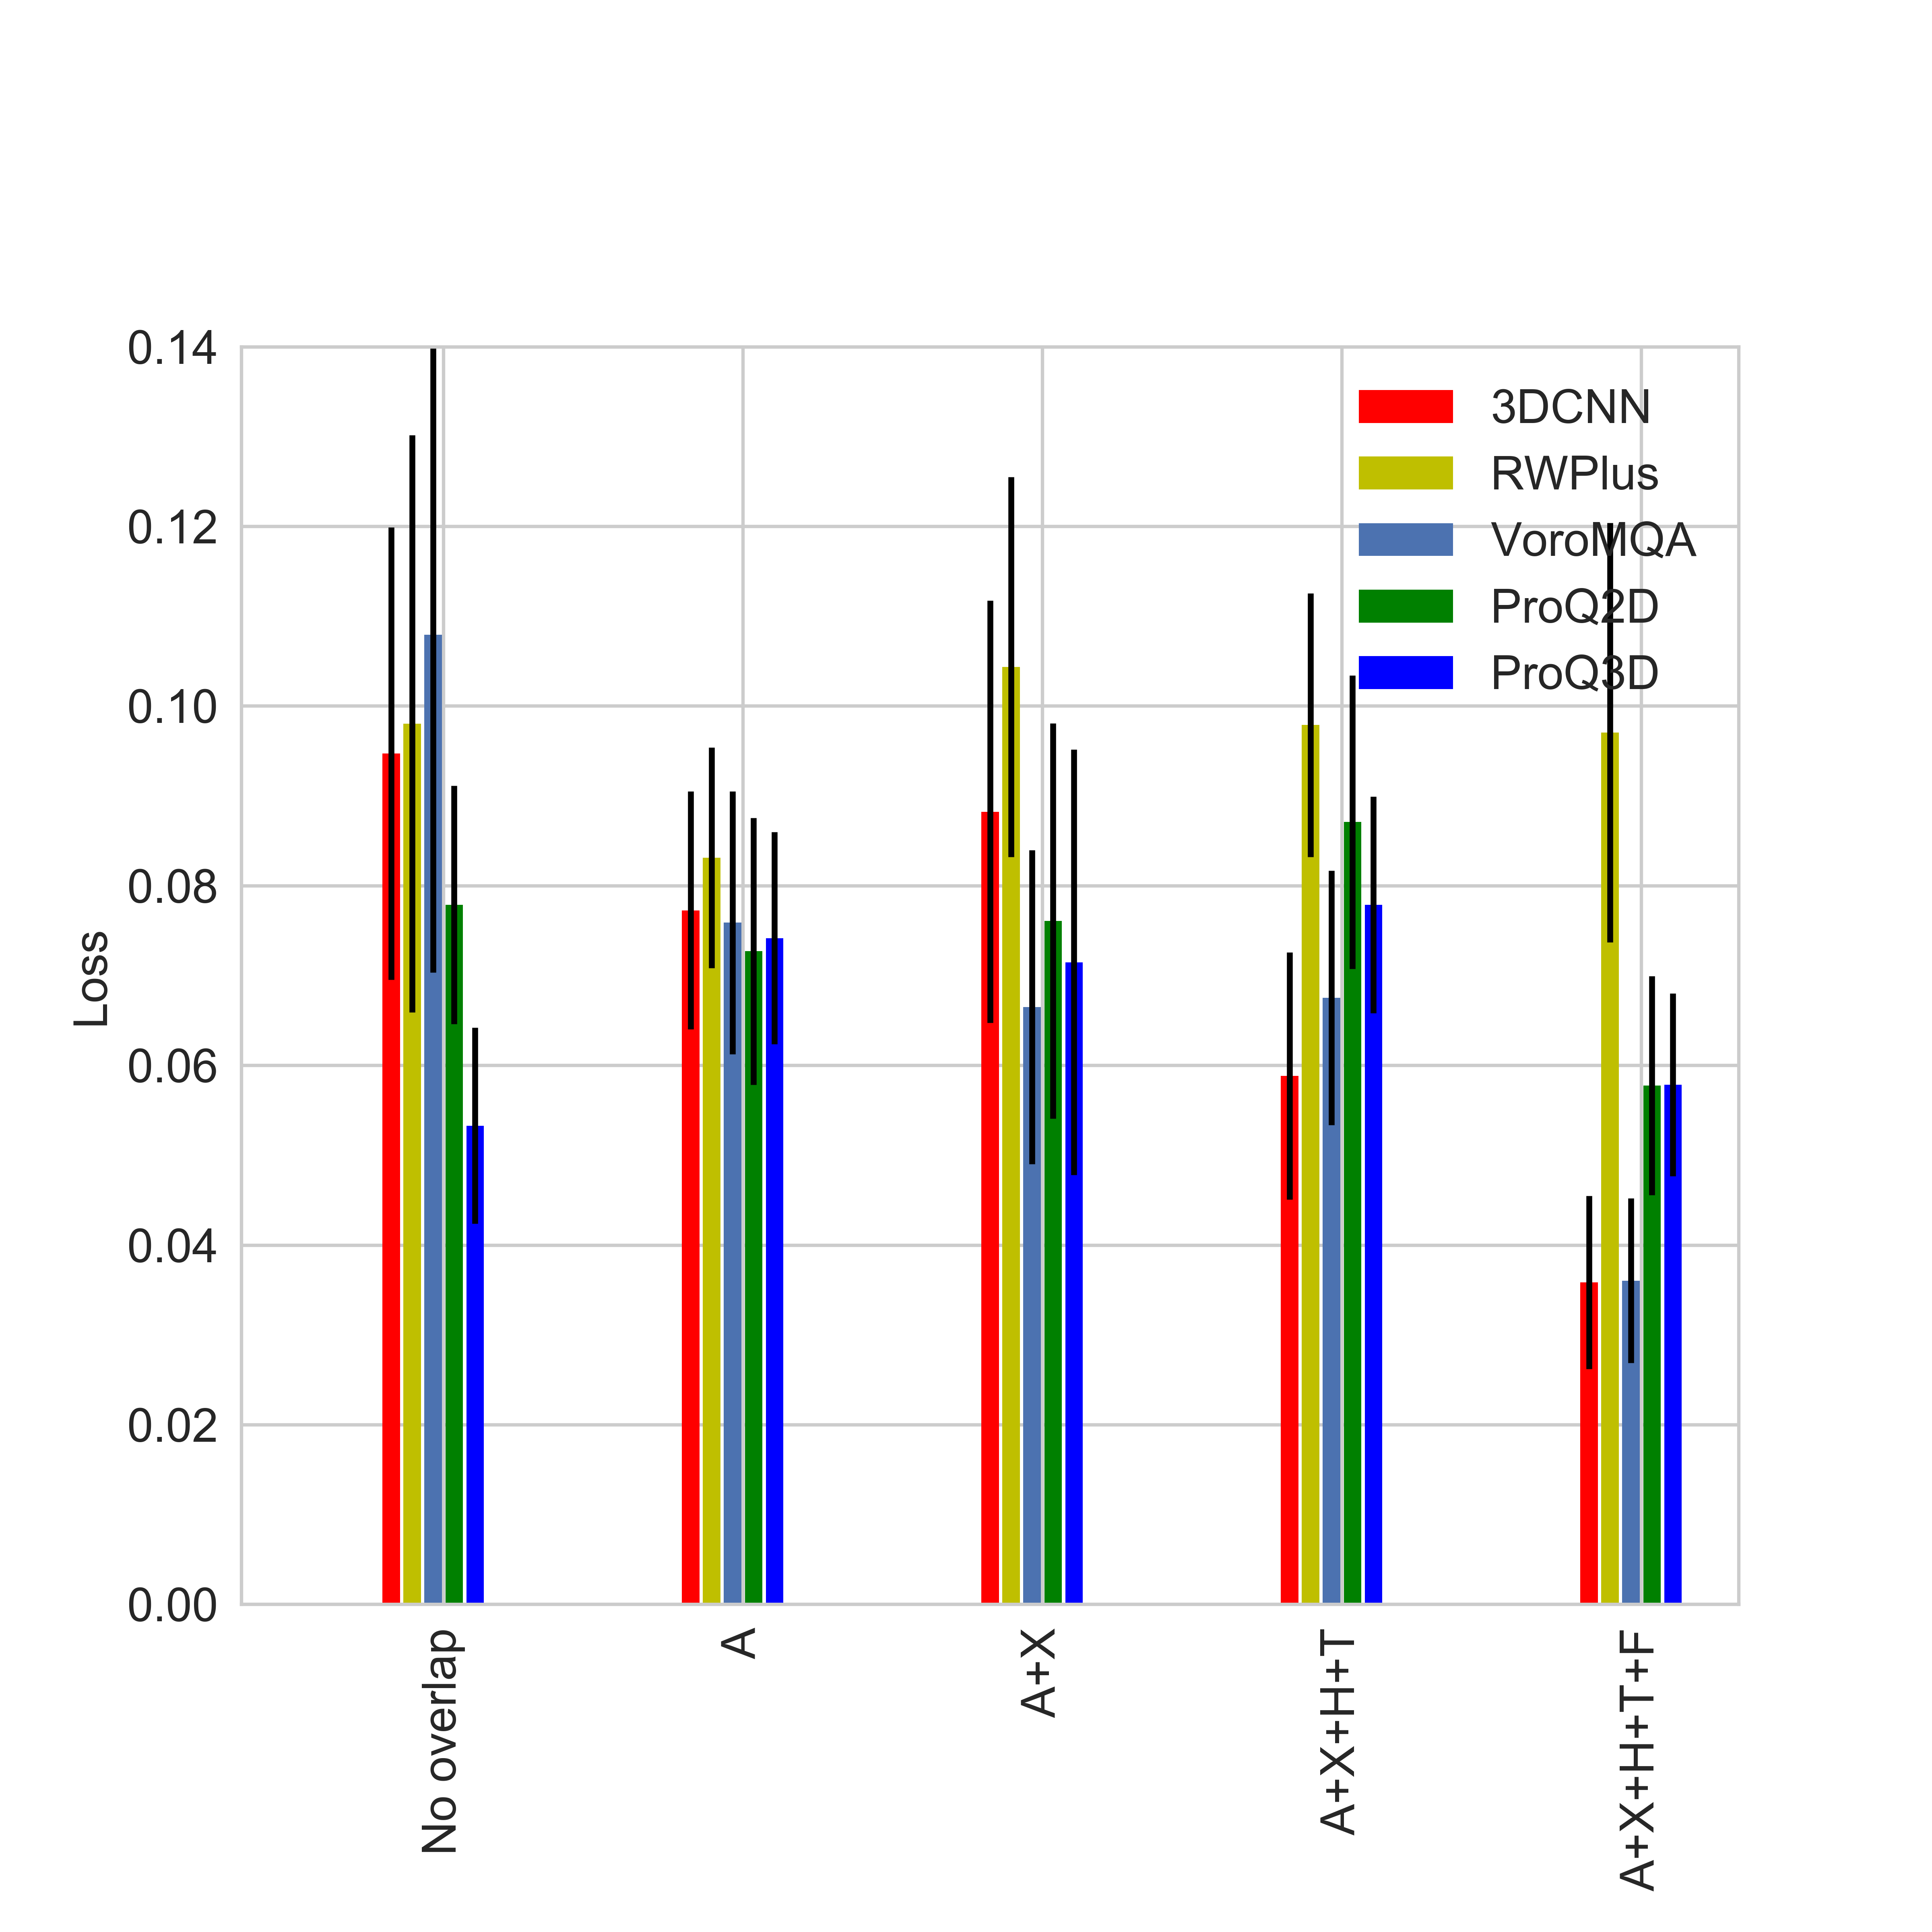
\includegraphics[width=\linewidth]{Fig/LossVsECOD.png}
%
    \caption{Per-target average loss of the MQA algorithms of Table~\ref{Tbl:TestResults}
    on the CASP11 test set stage~2, divided into 5 subsets of
    increasing structural similarity with the training set. The
    subsets are chosen according to the presence in the training set
    of structures belonging to the same ECOD categories (see text for
    details). Error bars show per-target standard deviation of the loss}
%
    \label{Fig:LossVsECOD}
\end{figure}


\begin{figure}[H]
    \centering
    \makebox[0pt][c]{
    \hskip-\footskip
    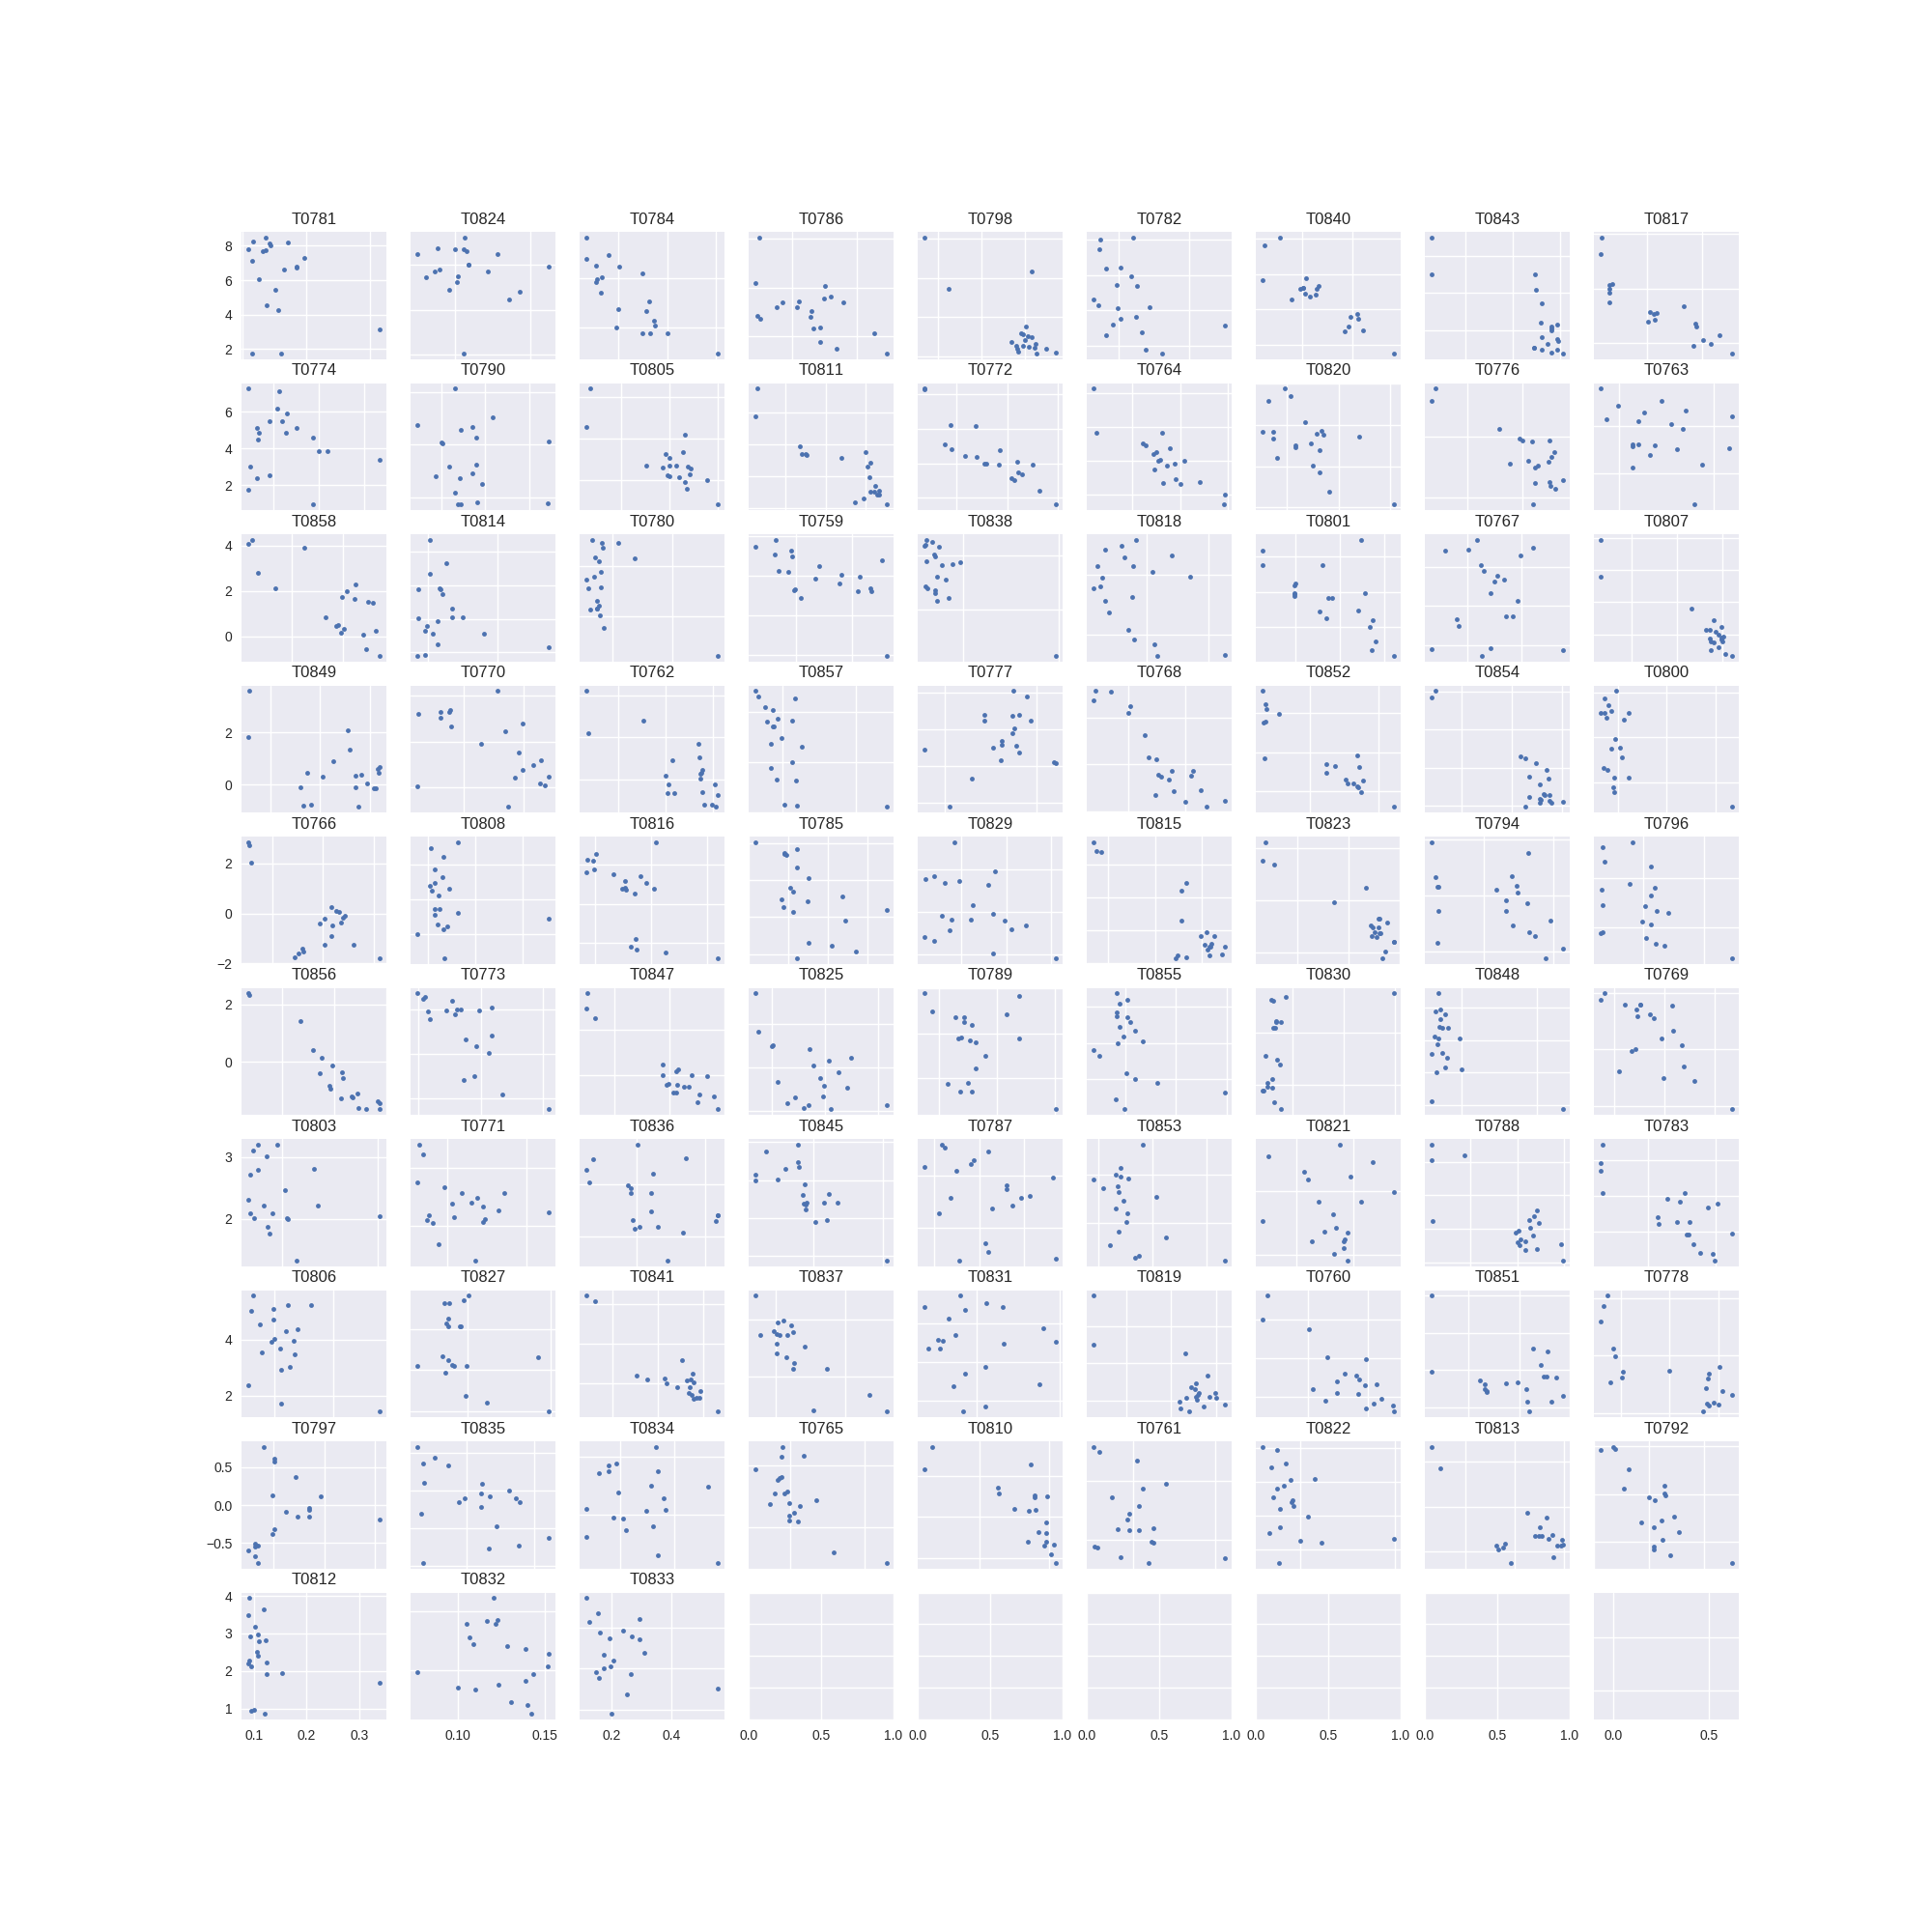
\includegraphics[width=\paperwidth]{Fig/CASP11Stage1_SCWRL_sFinal_funnels.png}
    \hskip\headheight
    }
    \caption{Scoring funnels on Stage1 CASP11}
    \label{Fig:Satage1CASP11Funnels}
\end{figure}

\begin{figure}[H]
    \centering
    \makebox[0pt][c]{
    \hskip-\footskip
    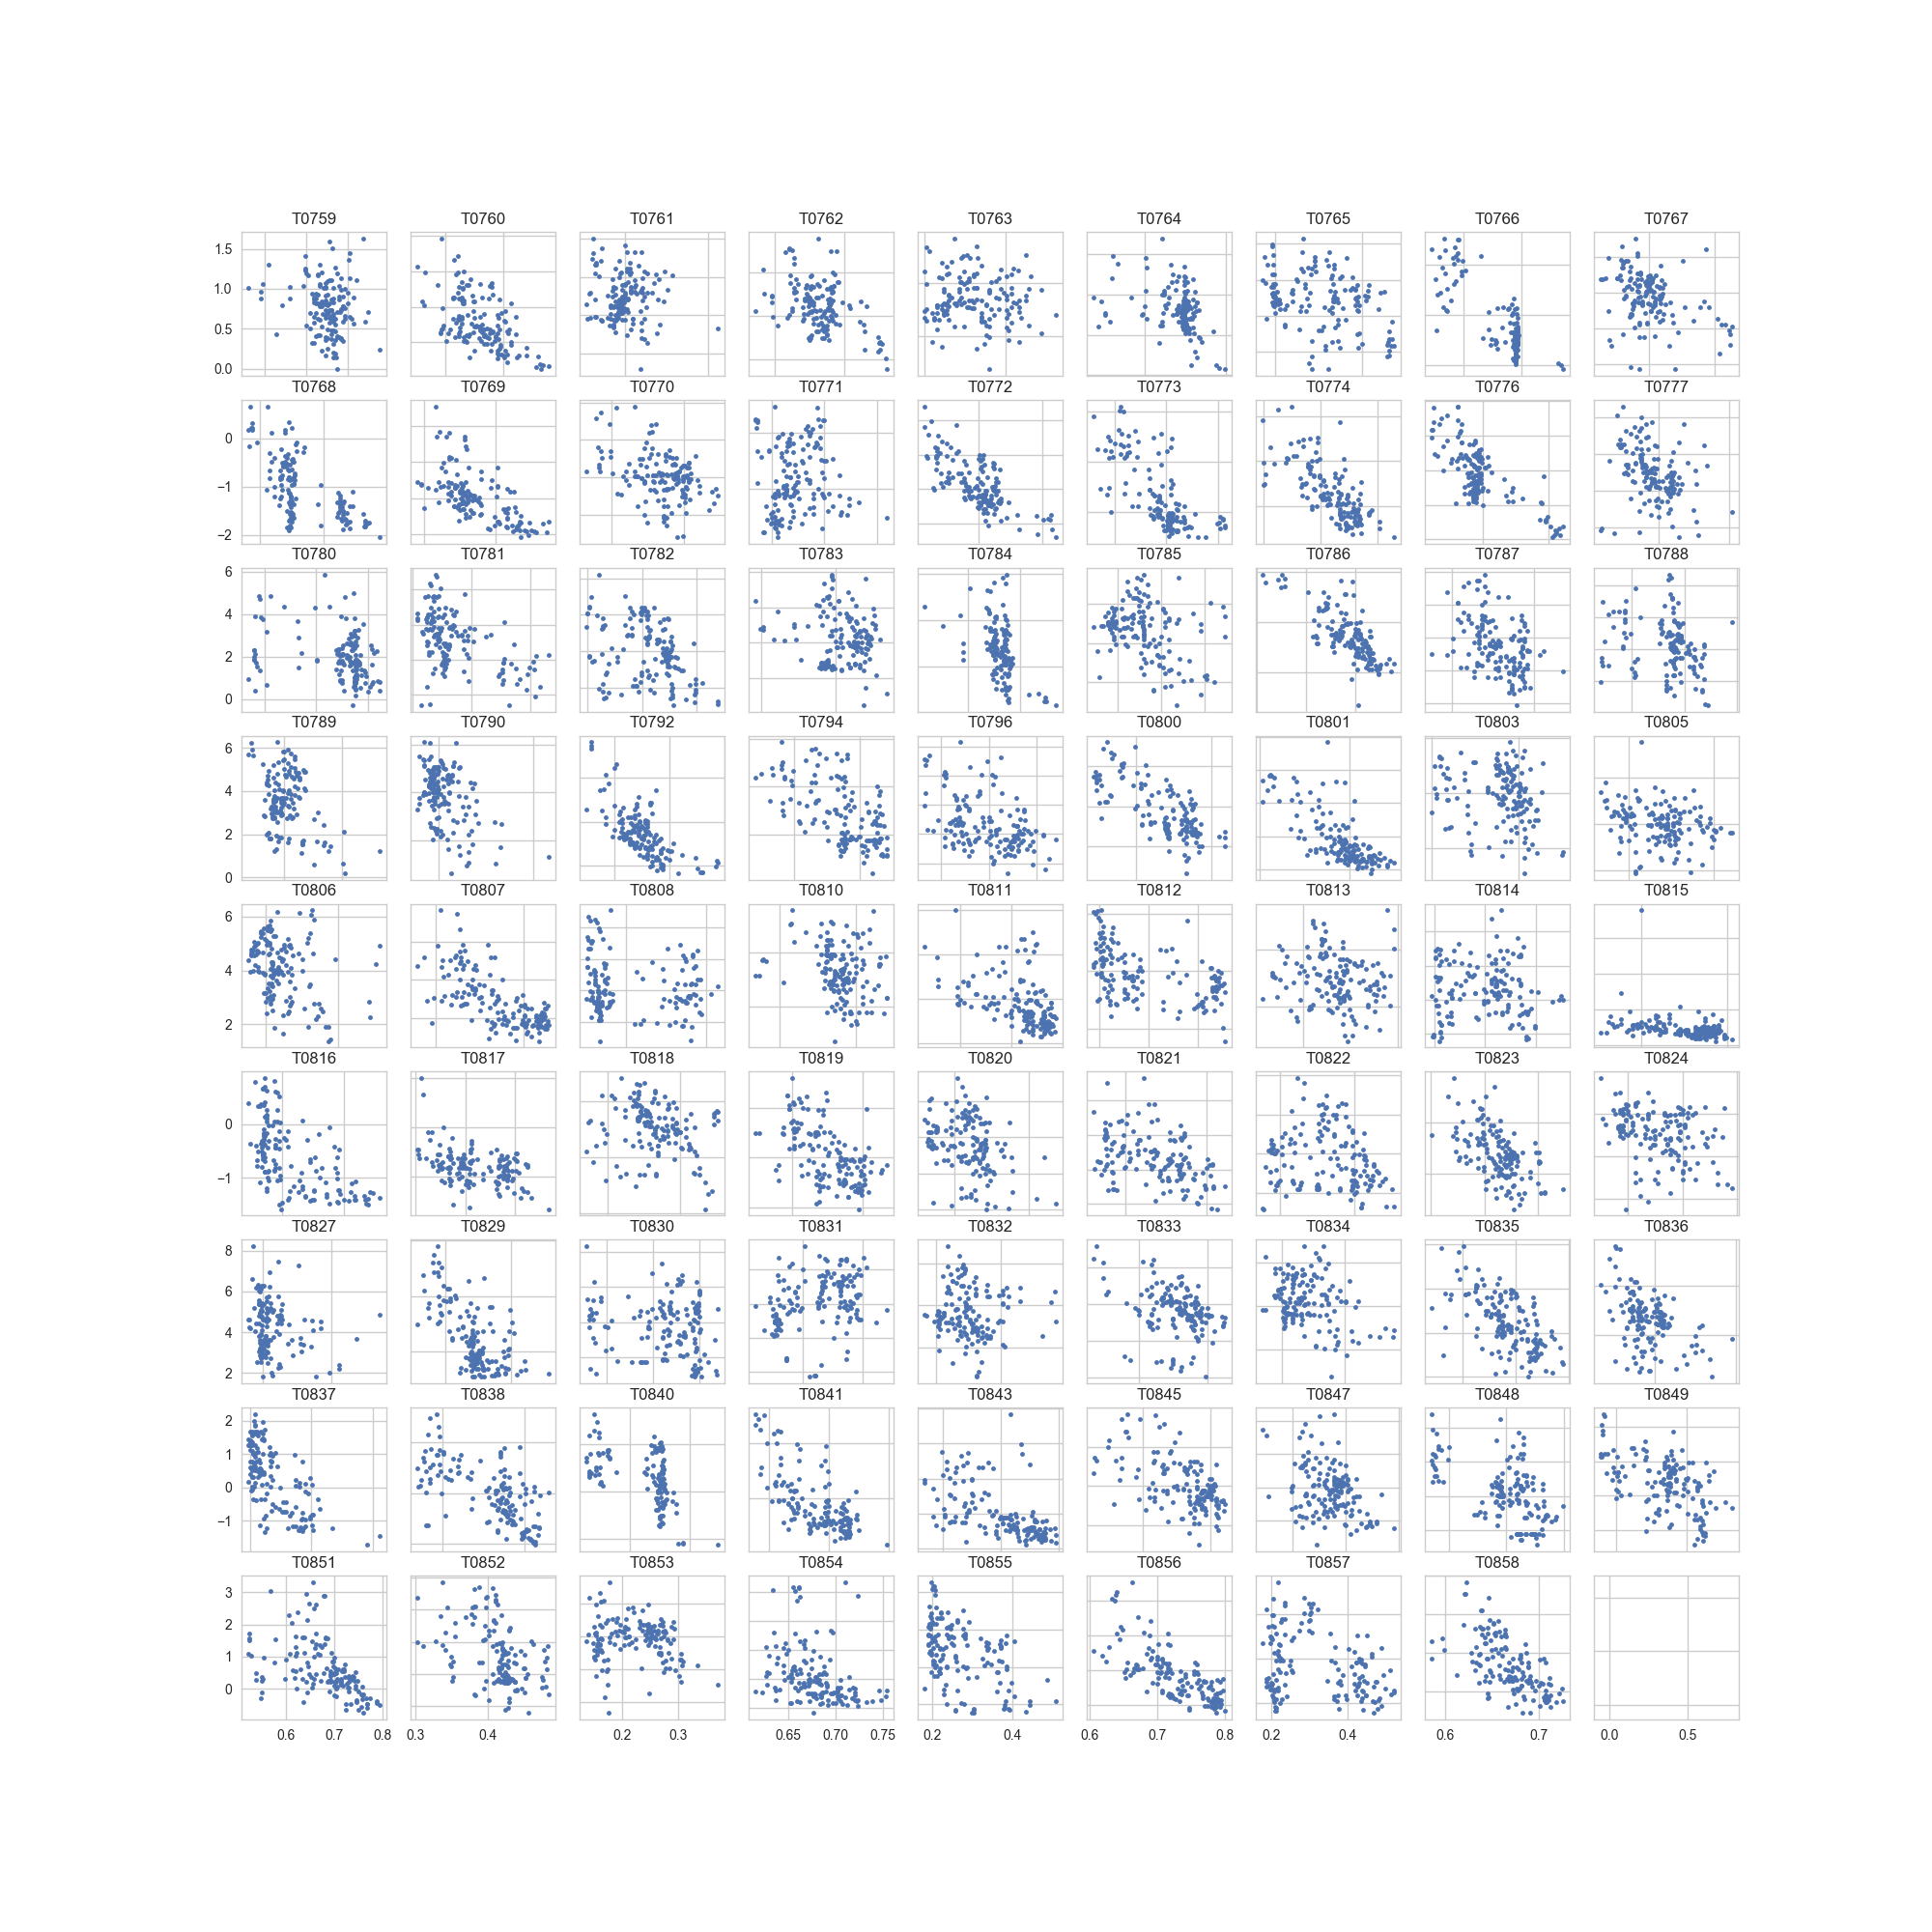
\includegraphics[width=\paperwidth]{Fig/CASP11Stage2_SCWRL_sFinal_funnels.png}
    \hskip\headheight
    }
    \caption{Scoring funnels on Stage2 CASP11}
    \label{Fig:Satage2CASP11Funnels}
\end{figure}

\section{Analysis}

\begin{figure}[H]
    \centering
    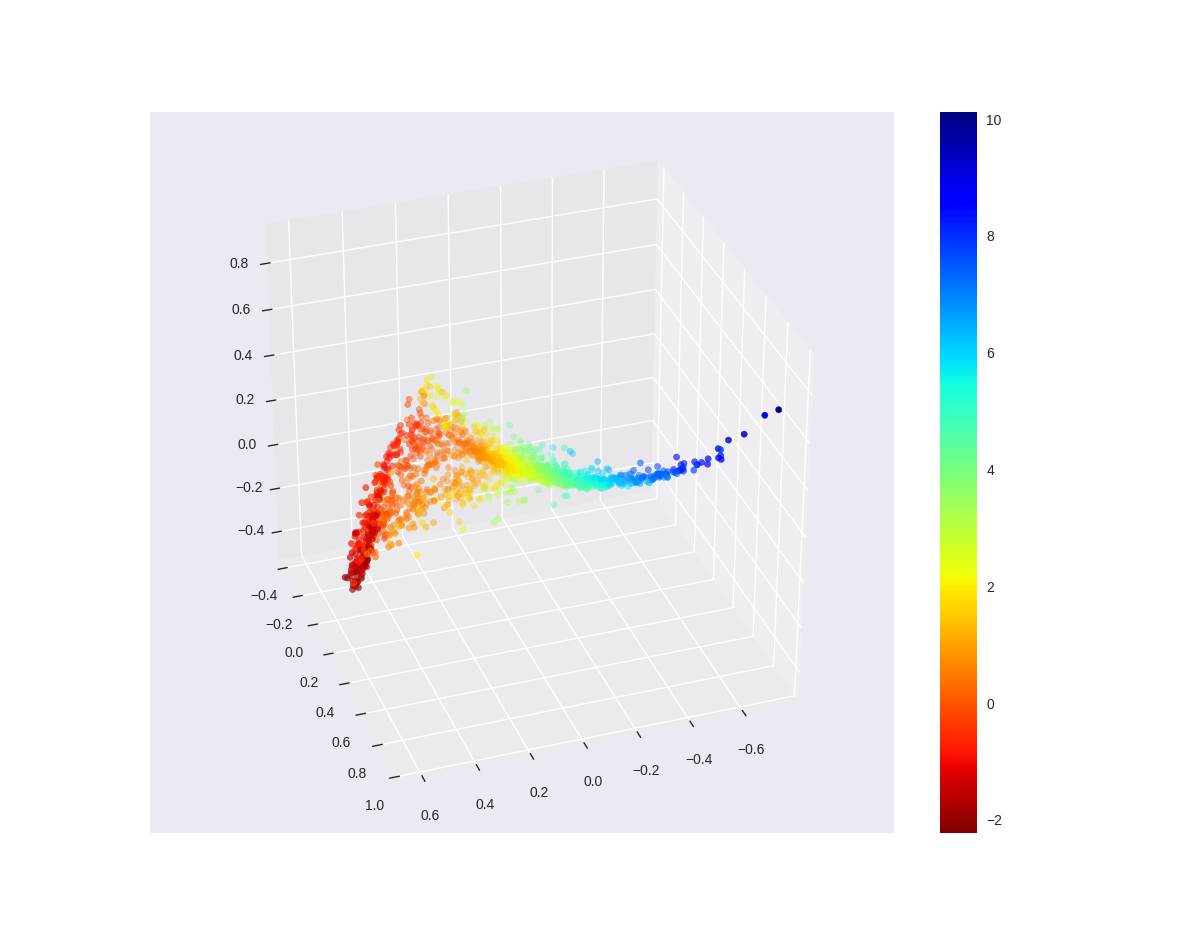
\includegraphics[width=\linewidth]{Fig/CASP11Stage1_SCWRL_activations_pca.png}
    \caption{First three principal components of layer 28 activations versus model score (color bar).}
    \label{Fig:PCA}
\end{figure}



\bibliography{citations.bib}{}
\bibliographystyle{plain}

\end{document}